\documentclass[11pt]{beamer}
\usetheme{Szeged}
\usepackage[utf8]{inputenc}
\usepackage{amsmath}
\usepackage{amsfonts}
\usepackage{amssymb}
\usepackage{graphicx}
\author{Miguel Tinta Aguilar, Angelo Figueroa Vega}
\title{Recursion}
\subtitle{Recursion}
%\setbeamercovered{transparent} 
%\setbeamertemplate{navigation symbols}{} 
%\logo{} 
\institute[UNSA]{
System Engineering School\\
System Engineering and Informatic Department\\
Production and Services Faculty\\
San Agustin National University of Arequipa} 
%\date{} 
\titlegraphic{
\includegraphics[width=3.0cm]{IMGS/logo_unsa.jpg}}
%\subject{} 
\begin{document}

\begin{frame}
\titlepage
\end{frame}

\begin{frame}
\tableofcontents
\end{frame}

\section{Definition}
\begin{frame}{•}
\frametitle{What is Recursion}
Recursion is a method of solving a problem where the solution depends on solutions to smaller instances of the same problem.
\\To do these tasks the recursion involves a function calling itself.
\end{frame}

\begin{frame}[fragile]
\frametitle{Example}
\begin{verbatim}
 static int factorial(int n){    
  if (n == 0)    
    return 1;    
  else    
    return(n * factorial(n-1));	//RECURSION
\end{verbatim}
\end{frame}

\section{How does it work}
\begin{frame}
\frametitle{How Recursive methods works}
To write a recursive method you need to know two parts:\\
A base case and a general case. The first one will make the recursive method reach an end, and the second one it is the operation.

\end{frame}
\begin{frame}[fragile]
\frametitle{Example}
\begin{verbatim}
 static int factorial(int n){    
  if (n == 0)    
    return 1;    				//BASE CASE
  else    
    return(n * factorial(n-1));	//GENERAL CASE
\end{verbatim}
\end{frame}
\begin{frame}
\frametitle{Graphic Representation}
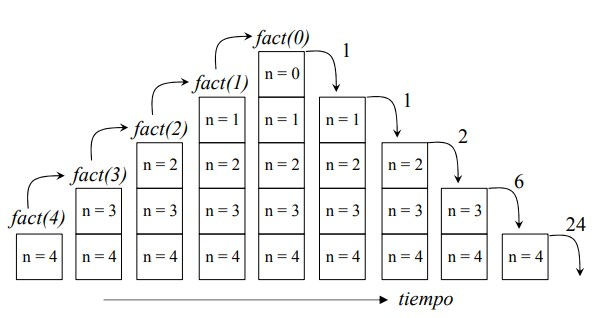
\includegraphics[scale=0.7]{IMGS/Screenshot_5.jpg} 
\end{frame}

\section{Recursion and Iteration}
\begin{frame}
\frametitle{Important aspects to be taken into consideration when using recursion and iteration}
\begin{itemize}
\item [The computing load] 
\begin{description}
Time of Ejecution and memory used.
\end{description}
\item [Redundancy]
\begin{description}
Sometimes Recursion resolves the same problem multiple times.
\end{description}
\item [Solution]
\begin{description}
Sometimes an iterative solution it is too complicate to find
\end{description}
\item [Resultant code]
\begin{description}
Using recursion, the final code might be more concise, elegant and easy to read and understand
\end{description}
\end{itemize}

\end{frame}
\begin{frame}[fragile]
\frametitle{Comparation between Recursion and Iteration}
Recursion
\begin{verbatim}
 static int factorial(int n){    
  if (n == 0)    
    return 1;    				
  else    
    return(n * factorial(n-1));	
\end{verbatim}
\end{frame}
\begin{frame}[fragile]
Iteration
\begin{verbatim}
public static int factorial(int n) {
		if (n == 0) {
			return 1;
		}else  {
			int factorial = 1;
			for(int i=1;i<=n;i++) {
				factorial = factorial * i;	
			}return factorial;
			}	}
\end{verbatim}
\end{frame}

\section{Fibbonaci}


\section{Utility}

\end{document}